% Date : 03/11/2022
% Version : 1
% Auteur : JJF
% Relu :
% Relecteur :

% ------------------------------------------------------------ %
% ----------------------  Fiche MCA04  ----------------------- %
% Thème : Moment cinétique
% Classes : PCSI, MPSI, PTSI, TSI, ATS
% ------------------------------------------------------------ %



% ======================================================= %
% ============== Gestion de la compilation ============== %
% ======================================================= %
\ifdefined\mainIsLoaded\else
\RequirePackage{import}
\subimport{../../}{_preambule_CdE_PC}
\begin{document}
\fi
% ======================================================= %
% ======================================================= %






% ============================================================================ %
%                            FICHE D'ENTRAÎNEMENT                              %
% ============================================================================ %
% ======================= Métadonnées sur la fiche =========================== %
\titreFicheEntrainement		{Moment cinétique}
\grandTheme					{Mécanique}
\numeroFiche				{MCA04}
\uniqueID					{eZZFHFuXSlD} % une chaîne de caractères (a-z, A-Z) aléatoire de 10 caractères.
\nombreColonnesReponses		{2} % 1, 2, 3, \etc{}
% ============================================================================ %

%%%%%%%%%%%%%%%%%%%%%%%%%%%%%%%%%%%%%%%%%%%%%%%%%%%%%%%%%%%%%%%%%%%%%%%%%%
\debutFicheEntrainement                                                  %
%%%%%%%%%%%%%%%%%%%%%%%%%%%%%%%%%%%%%%%%%%%%%%%%%%%%%%%%%%%%%%%%%%%%%%%%%%




% --------------------------------------------------------------------- %
%                              Prérequis                                %
%                             (facultatif)                              %
% --------------------------------------------------------------------- %
% ================== Métadonnées sur le prérequis ===================== %
\avecPrerequis{Y} % Y ou N
% ====================================== %
\begin{prerequis}
	Coordonnées polaires. Projections. Produit vectoriel. Moment cinétique. Moment d'inertie. Moment d'une force.
\end{prerequis}
% --------------------------------------------------------------------- %




% •••••••••••••••••••••••••••••••••••••••••••••••••••••••••••••••••••••••••••• %
% •••••••••••••••••••••••••••••••••••••••••••••••••••••••••••••••••••••••••••• %
\sectionFicheEntrainement{Projections préparatoires}
% •••••••••••••••••••••••••••••••••••••••••••••••••••••••••••••••••••••••••••• %
% •••••••••••••••••••••••••••••••••••••••••••••••••••••••••••••••••••••••••••• %



% ************************************** %
%             ENTRAÎNEMENT               %
% ************************************** %
% === Métadonnées sur l'entraînement === %

\titreEntrainementFacultatif	{Calculs de produits scalaires}
\hauteurLargeurCadreReponse		{8mm}{3cm}
\dureeResolutionFacultative		{2} % 1, 2, 3 ou 4
\typeEntrainement				{Newton} % Newton ou QCM ou AN ou vide (exercice "normal")
\basiqueEtTransversal			{Y}
\nombreColonnesQuestions		{3} % vide, 1, 2, 3, \etc{}
\avecPlusieursQuestions			{Y} % Y ou N
\initialisationEntrainement
% ====================================== %

On considère les vecteurs suivants où $\vv{P}$ et $\vv{T}$ sont verticaux.
\label{schema:projections}

\hfil
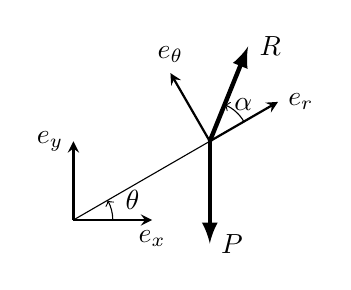
\begin{tikzpicture}
	\draw [-stealth,thick]  (0,0) -- (0,1) node [left] {$\vv{e_y}$};
  \draw [-stealth,thick]  (0,0) -- (1,0) node [below] {$\vv{e_x}$};
   \pgfmathsetmacro{\THETA}{30}
	 \pgfmathsetmacro{\ALPHA}{38}
   \pgfmathsetmacro{\cosTHETA}{cos(\THETA)}
   \pgfmathsetmacro{\sinTHETA}{sin(\THETA)}
	 \pgfmathsetmacro{\cosALPHA}{cos(\ALPHA)}
	 \pgfmathsetmacro{\sinALPHA}{sin(\ALPHA)}
  \draw [-stealth,thick,rotate=\THETA]  (2,0) -- (2,1) node [above] {$\vv{e_\theta}$};
	\draw [-latex,\blueOrBlack,ultra thick,rotate=\THETA]  (2,0) -- (2+1.3*\cosALPHA,1.3*\sinALPHA) node [right] {$\vv{R}$};
  \draw [->,rotate=\THETA]  (2.5,0) arc (0:\ALPHA:0.5) node [right] {$\alpha$};
  \draw [-stealth,thick,rotate=\THETA]  (2,0) -- (3,0) node [right] {$\vv{e_r}$};
  \draw [-latex,\blueOrBlack,ultra thick]  (2*\cosTHETA,2*\sinTHETA) -- (2*\cosTHETA,2*\sinTHETA-1.3) node [right] {$\vv{P}$};
  \draw [rotate=\THETA] (0,0) -- (2,0) ;
  \draw [->] (0.5,0) arc (0:\THETA:0.5) node [right=3pt] {$\theta$};
\end{tikzpicture}\hfil
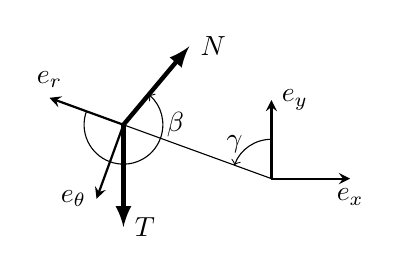
\begin{tikzpicture}
	  \draw [-stealth,thick]  (0,0) -- (0,1) node [right] {$\vv{e_y}$};
	  \draw [-stealth,thick]  (0,0) -- (1,0) node [below] {$\vv{e_x}$};
	   \pgfmathsetmacro{\THETA}{160}
	   \pgfmathsetmacro{\ALPHA}{250}
	   \pgfmathsetmacro{\cosTHETA}{cos(\THETA)}
	   \pgfmathsetmacro{\sinTHETA}{sin(\THETA)}
	   \pgfmathsetmacro{\cosALPHA}{cos(\ALPHA)}
	   \pgfmathsetmacro{\sinALPHA}{sin(\ALPHA)}
	  \draw [-stealth,thick,rotate=\THETA]  (2,0) -- (2,1) node [left] {$\vv{e_\theta}$};
	  \draw [->,rotate=\THETA]  (2.5,0) arc (0:\ALPHA:0.5) node [below right=3pt] {$\beta$};
	  \draw [-stealth,thick,rotate=\THETA]  (2,0) -- (3,0) node [above] {$\vv{e_r}$};
	  \draw [-latex,\blueOrBlack,ultra thick,rotate=\THETA]  (2,0) -- (2+1.3*\cosALPHA,1.3*\sinALPHA) node [right] {$\vv{N}$};
	  \draw [-latex,\blueOrBlack,ultra thick]  (2*\cosTHETA,2*\sinTHETA) -- (2*\cosTHETA,2*\sinTHETA-1.3) node [right] {$\vv{T}$};
	  \draw [rotate=\THETA] (0,0) -- (2,0) ;
	  \draw [->] (0,0.5) arc (90:\THETA:0.5) node [above=1pt] {$\gamma$};
\end{tikzpicture}

Calculer les produits scalaires suivants en fonction des normes ($\Arrowvert\vv{P}\Arrowvert$, $\Arrowvert\vv{T}\Arrowvert$, \etc{}) ainsi que des différents angles apparaissant sur les schémas.

% ====================================== %
\debutEntrainement
% ====================================== %

% ^^^^^^^^^^^^^^^^^^^^^^^^^^^^^^^^^^^^^^ %
%               Question                 %
% ^^^^^^^^^^^^^^^^^^^^^^^^^^^^^^^^^^^^^^ %

\begin{enonce}
$\vv{P}\cdot\vv{e_\theta}$
\end{enonce}

\reponse{$-\Arrowvert\vv{P}\Arrowvert\,\cos\theta$}

\begin{corrige}
	On calcule $\vv{P}\cdot\vv{e_\theta}
		= \Arrowvert\vv{P}\Arrowvert\times
			\Arrowvert\vv{e_\theta}\Arrowvert\times
			\cos(\pi + \theta)
		= -\Arrowvert\vv{P}\Arrowvert\,\cos\theta$.
\end{corrige}

% ************************************** %


% ^^^^^^^^^^^^^^^^^^^^^^^^^^^^^^^^^^^^^^ %
%               Question                 %
% ^^^^^^^^^^^^^^^^^^^^^^^^^^^^^^^^^^^^^^ %

\begin{enonce}
$\vv{N}\cdot\vv{e_y}$
\end{enonce}

\reponse{$\Arrowvert\vv{N}\Arrowvert\,\cos(\gamma + \beta)$}

% ************************************** %


% ^^^^^^^^^^^^^^^^^^^^^^^^^^^^^^^^^^^^^^ %
%               Question                 %
% ^^^^^^^^^^^^^^^^^^^^^^^^^^^^^^^^^^^^^^ %

\begin{enonce}
$\vv{R}\cdot\vv{e_y}$
\end{enonce}

\reponse{$\Arrowvert\vv{R}\Arrowvert\,\sin(\theta + \alpha)$}

\begin{corrige}
	On calcule $\vv{R}\cdot\vv{e_y}
		= \Arrowvert\vv{R}\Arrowvert\times
			\Arrowvert\vv{e_y}\Arrowvert\times
			\cos\left(\frac{\pi}{2} - (\theta + \alpha)\right)
		= \Arrowvert\vv{R}\Arrowvert\,\sin(\theta + \alpha)$.
\end{corrige}

% ************************************** %


% ^^^^^^^^^^^^^^^^^^^^^^^^^^^^^^^^^^^^^^ %
%               Question                 %
% ^^^^^^^^^^^^^^^^^^^^^^^^^^^^^^^^^^^^^^ %

\begin{enonce}
$\vv{T}\cdot\vv{e_r}$
\end{enonce}

\reponse{$-\Arrowvert\vv{T}\Arrowvert\,\cos(\gamma)$}

\begin{corrige}
	On calcule $\vv{T}\cdot\vv{e_r}
		= \Arrowvert\vv{T}\Arrowvert\times
			\Arrowvert\vv{e_r}\Arrowvert\times
			\cos(\pi + \gamma)
		= -\Arrowvert\vv{T}\Arrowvert\,\cos(\gamma)$.
\end{corrige}

% ************************************** %



% ^^^^^^^^^^^^^^^^^^^^^^^^^^^^^^^^^^^^^^ %
%               Question                 %
% ^^^^^^^^^^^^^^^^^^^^^^^^^^^^^^^^^^^^^^ %

\begin{enonce}
$\vv{N}\cdot\vv{e_r}$
\end{enonce}

\reponse{$\Arrowvert\vv{N}\Arrowvert\,\cos(\beta)$}

% ************************************** %


% ^^^^^^^^^^^^^^^^^^^^^^^^^^^^^^^^^^^^^^ %
%               Question                 %
% ^^^^^^^^^^^^^^^^^^^^^^^^^^^^^^^^^^^^^^ %

\begin{enonce}
$\vv{N}\cdot\vv{e_\theta}$
\end{enonce}

\reponse{$\Arrowvert\vv{N}\Arrowvert\,\sin(\beta)$}

\begin{corrige}
	On calcule $\vv{N}\cdot\vv{e_\theta}
		= \Arrowvert\vv{N}\Arrowvert\times
			\Arrowvert\vv{e_\theta}\Arrowvert\times
			\cos\left(\beta - \frac\pi2\right)
		= \Arrowvert\vv{N}\Arrowvert\,\sin(\beta)$.
\end{corrige}

% ************************************** %

% ====================================== %
\finEntrainement
% ====================================== %






% ************************************** %
%             ENTRAÎNEMENT               %
% ************************************** %
% === Métadonnées sur l'entraînement === %

\titreEntrainementFacultatif	{Projections dans une base}
\hauteurLargeurCadreReponse		{10mm}{4.5cm}
\dureeResolutionFacultative		{2} % 1, 2, 3 ou 4
\typeEntrainement				{Newton} % Newton ou QCM ou AN ou vide (exercice "normal")
\basiqueEtTransversal			{Y}
\nombreColonnesQuestions		{2} % vide, 1, 2, 3, \etc{}
\avecPlusieursQuestions			{Y} % Y ou N
\initialisationEntrainement
% ====================================== %

En utilisant la formule donnant la décomposition d'un vecteur $\vv{v}$ dans une base orthonormée $(\vv{e_1},\vv{e_2})$
\[
\vv{v} = (\vv{v}\cdot\vv{e_1})\;\vv{e_1} +
					(\vv{v}\cdot\vv{e_2})\;\vv{e_2},
					\]
décomposer les vecteurs de l'exercice précédent dans chaque base $(\vv{e_x},\vv{e_y})$ et $(\vv{e_r},\vv{e_\theta})$.\label{decompositions}

% ====================================== %
\debutEntrainement
% ====================================== %

% ^^^^^^^^^^^^^^^^^^^^^^^^^^^^^^^^^^^^^^ %
%               Question                 %
% ^^^^^^^^^^^^^^^^^^^^^^^^^^^^^^^^^^^^^^ %

\begin{enonce}
$\vv{P}$ dans $(\vv{e_x}, \vv{e_y})$
\end{enonce}

\reponse{$\vv{P} =
-\Arrowvert\vv{P}\Arrowvert\,\vv{e_y}
$}

% ************************************** %

% ^^^^^^^^^^^^^^^^^^^^^^^^^^^^^^^^^^^^^^ %
%               Question                 %
% ^^^^^^^^^^^^^^^^^^^^^^^^^^^^^^^^^^^^^^ %

\begin{enonce}
$\vv{P}$ dans $(\vv{e_r}, \vv{e_\theta})$
\end{enonce}

\reponse{$
\Arrowvert\vv{P}\Arrowvert\left(
	-\sin(\theta)\,\vv{e_r} - \cos(\theta)\,\vv{e_\theta}
\right)$}

% ************************************** %

% ^^^^^^^^^^^^^^^^^^^^^^^^^^^^^^^^^^^^^^ %
%               Question                 %
% ^^^^^^^^^^^^^^^^^^^^^^^^^^^^^^^^^^^^^^ %

\begin{enonce}
$\vv{T}$ dans $(\vv{e_x}, \vv{e_y})$
\end{enonce}

\reponse{$
-\Arrowvert\vv{T}\Arrowvert\vv{e_y}
$}

% ************************************** %

% ^^^^^^^^^^^^^^^^^^^^^^^^^^^^^^^^^^^^^^ %
%               Question                 %
% ^^^^^^^^^^^^^^^^^^^^^^^^^^^^^^^^^^^^^^ %

\begin{enonce}
$\vv{T}$ dans $(\vv{e_r}, \vv{e_\theta})$
\end{enonce}

\reponse{$\vv{T} =
\Arrowvert\vv{T}\Arrowvert\left(
	-\cos(\gamma)\,\vv{e_r} + \sin(\gamma)\,\vv{e_\theta}
\right)$}

% ************************************** %

% ^^^^^^^^^^^^^^^^^^^^^^^^^^^^^^^^^^^^^^ %
%               Question                 %
% ^^^^^^^^^^^^^^^^^^^^^^^^^^^^^^^^^^^^^^ %

\begin{enonce}
$\vv{R}$ dans $(\vv{e_x}, \vv{e_y})$
\end{enonce}

\reponse{$
\Arrowvert\vv{R}\Arrowvert\left(
	\cos(\theta+\alpha)\,\vv{e_x} + \sin(\theta+\alpha)\,\vv{e_y}
\right)$}

% ************************************** %

% ^^^^^^^^^^^^^^^^^^^^^^^^^^^^^^^^^^^^^^ %
%               Question                 %
% ^^^^^^^^^^^^^^^^^^^^^^^^^^^^^^^^^^^^^^ %

\begin{enonce}
$\vv{R}$ dans $(\vv{e_r}, \vv{e_\theta})$
\end{enonce}

\reponse{$
\Arrowvert\vv{R}\Arrowvert\left(
	\cos(\alpha)\,\vv{e_r} + \sin(\alpha)\,\vv{e_\theta}
\right)$}

% ************************************** %

% ^^^^^^^^^^^^^^^^^^^^^^^^^^^^^^^^^^^^^^ %
%               Question                 %
% ^^^^^^^^^^^^^^^^^^^^^^^^^^^^^^^^^^^^^^ %

\begin{enonce}
$\vv{N}$ dans $(\vv{e_x}, \vv{e_y})$
\end{enonce}

\reponse{$
\Arrowvert\vv{N}\Arrowvert\left(
	-\sin(\beta+\gamma)\,\vv{e_x} + \cos(\gamma+\beta)\,\vv{e_y}
\right)$}

% ************************************** %

% ^^^^^^^^^^^^^^^^^^^^^^^^^^^^^^^^^^^^^^ %
%               Question                 %
% ^^^^^^^^^^^^^^^^^^^^^^^^^^^^^^^^^^^^^^ %

\begin{enonce}
$\vv{N}$ dans $(\vv{e_r}, \vv{e_\theta})$
\end{enonce}

\reponse{$
\Arrowvert\vv{N}\Arrowvert\left(
	\cos(\beta)\,\vv{e_r} + \sin(\beta)\,\vv{e_\theta}
\right)$}

% ************************************** %

% ====================================== %
\finEntrainement
% ====================================== %




% •••••••••••••••••••••••••••••••••••••• %
% •••••••••••••••••••••••••••••••••••••• %
\sectionFicheEntrainement{Produit vectoriel}
% •••••••••••••••••••••••••••••••••••••• %
% •••••••••••••••••••••••••••••••••••••• %



% ************************************** %
%             ENTRAÎNEMENT               %
% ************************************** %
% === Métadonnées sur l'entraînement === %

\titreEntrainementFacultatif	{Produits vectoriels à partir de décompositions}
\hauteurLargeurCadreReponse		{8mm}{2.7cm}
\dureeResolutionFacultative		{1} % 1, 2, 3 ou 4
\typeEntrainement				{Newton} % Newton ou QCM ou AN ou vide (exercice "normal")
\basiqueEtTransversal			{Y}
\nombreColonnesQuestions		{3} % vide, 1, 2, 3, \etc{}
\avecPlusieursQuestions			{Y} % Y ou N
\initialisationEntrainement
% ====================================== %

En utilisant le schéma du premier exercice et les décompositions du deuxième, donner l'expression des produits vectoriels suivants. Comme d'habitude, on complète la base $(\vv{e_x}, \vv{e_y})$ par le vecteur $\vv{e_z}$ suivant la \glm{règle de la main droite}.

% ====================================== %
\debutEntrainement
% ====================================== %

% ^^^^^^^^^^^^^^^^^^^^^^^^^^^^^^^^^^^^^^ %
%               Question                 %
% ^^^^^^^^^^^^^^^^^^^^^^^^^^^^^^^^^^^^^^ %

\begin{enonce}
$\vv{P} \wedge \vv{R}$
\end{enonce}

\reponse{$
\Arrowvert\vv{P}\Arrowvert\,
\Arrowvert\vv{R}\Arrowvert\cos(\theta+\alpha)
\,\vv{e_z}
$}

\begin{corrige}
On calcule $
\vv{P} \wedge \vv{R}
	= -\Arrowvert\vv{P}\Arrowvert\,\vv{e_y}
		\wedge
		\Arrowvert\vv{R}\Arrowvert\left(
			\cos(\theta+\alpha)\,\vv{e_x} + \sin(\theta+\alpha)\,\vv{e_y}
		\right)
	= - \Arrowvert\vv{P}\Arrowvert\,
			\Arrowvert\vv{R}\Arrowvert
			\cos(\theta+\alpha)\,\vv{e_y}\wedge\vv{e_x} + \vv{0}
%	= \Arrowvert\vv{P}\Arrowvert\,
%			\Arrowvert\vv{R}\Arrowvert
%			\cos(\theta+\alpha) \,\vv{e_z}
$.
\end{corrige}

% ************************************** %



% ^^^^^^^^^^^^^^^^^^^^^^^^^^^^^^^^^^^^^^ %
%               Question                 %
% ^^^^^^^^^^^^^^^^^^^^^^^^^^^^^^^^^^^^^^ %

\begin{enonce}
$\vv{T} \wedge \vv{e_r}$
\end{enonce}

\reponse{$
-\Arrowvert\vv{T}\Arrowvert\sin(\gamma)
\,\vv{e_z}
$}


\begin{corrige}
On calcule $
\vv{T} \wedge \vv{e_r}
	= \Arrowvert\vv{T}\Arrowvert\left(
		-\cos(\gamma)\,\vv{e_r} + \sin(\gamma)\,\vv{e_\theta}\right)
		\wedge
		\vv{e_r}
	= \Arrowvert\vv{T}\Arrowvert
		\sin(\gamma)\,\vv{e_\theta}\wedge\vv{e_r}
	= -\Arrowvert\vv{T}\Arrowvert\sin(\gamma)
	\,\vv{e_z}
$.
\end{corrige}

% ************************************** %


% ^^^^^^^^^^^^^^^^^^^^^^^^^^^^^^^^^^^^^^ %
%               Question                 %
% ^^^^^^^^^^^^^^^^^^^^^^^^^^^^^^^^^^^^^^ %

\begin{enonce}
$\vv{e_x} \wedge \vv{N}$
\end{enonce}

\reponse{$
\Arrowvert\vv{N}\Arrowvert\cos(\gamma+\beta)
\,\vv{e_z}
$}

\begin{corrige}
On calcule $
\vv{e_x} \wedge \vv{N}
	= \vv{e_x} \wedge
	\Arrowvert\vv{N}\Arrowvert\left(
		-\sin(\beta+\gamma)\,\vv{e_x} + \cos(\gamma+\beta)\,\vv{e_y}
	\right)
	= \Arrowvert\vv{N}\Arrowvert
		\cos(\gamma+\beta)\,\vv{e_x}\wedge\vv{e_y}
$.
\end{corrige}

% ************************************** %

% ====================================== %
\finEntrainement
% ====================================== %






% ************************************** %
%             ENTRAÎNEMENT               %
% ************************************** %
% === Métadonnées sur l'entraînement === %

\titreEntrainementFacultatif	{Produits vectoriels à partir des coordonnées}
\hauteurLargeurCadreReponse		{17mm}{1.8cm}
\dureeResolutionFacultative		{2} % 1, 2, 3 ou 4
\typeEntrainement				{AN} % Newton ou QCM ou AN ou vide (exercice "normal")
\basiqueEtTransversal			{Y}
\nombreColonnesQuestions		{2} % vide, 1, 2, 3, \etc{}
\avecPlusieursQuestions			{Y} % Y ou N
\initialisationEntrainement
% ====================================== %

On donne les quatre vecteurs suivants de $\R^3$ définis de manière numérique:
\[
\vv{A} = \begin{pmatrix}
1	\\ 2 \\ 3
\end{pmatrix},
\qquad
\vv{B} = \begin{pmatrix}
6 \\ 5 \\ 4
\end{pmatrix},
\qquad
\vv{C} = \begin{pmatrix}
0 \\ 1 \\ -1
\end{pmatrix}\qquad\text{et}\qquad
\vv{e_x} = \begin{pmatrix}
1 \\ 0 \\ 0
\end{pmatrix}.
\]

Calculer les produits vectoriels et produits scalaires suivant : 

% ====================================== %
\debutEntrainement
% ====================================== %

% ^^^^^^^^^^^^^^^^^^^^^^^^^^^^^^^^^^^^^^ %
%               Question                 %
% ^^^^^^^^^^^^^^^^^^^^^^^^^^^^^^^^^^^^^^ %

\begin{enonce}
$\vv{A}\wedge\vv{B}$
\end{enonce}

\reponse{$\small
\begin{pmatrix}
	-7 \\ 14 \\ -7
\end{pmatrix}
$}

\begin{corrige}
	On calcule $
	\begin{pmatrix}
		1	\\ 2 \\ 3
	\end{pmatrix} \wedge
	\begin{pmatrix}
		6 \\ 5 \\ 4
	\end{pmatrix}
	=
	\begin{pmatrix}
		2\times4 - 3\times 5 \\
		3\times6 - 1\times4	\\
		1\times5 - 2\times6
	\end{pmatrix}
	=
	\begin{pmatrix}
		-7 \\ 14 \\ -7
	\end{pmatrix}
	$.
\end{corrige}

% ************************************** %


% ^^^^^^^^^^^^^^^^^^^^^^^^^^^^^^^^^^^^^^ %
%               Question                 %
% ^^^^^^^^^^^^^^^^^^^^^^^^^^^^^^^^^^^^^^ %

\begin{enonce}
$(\vv{B} + \vv{A})\wedge\vv{A}$
\end{enonce}

\reponse{$\small
\begin{pmatrix}
	7 \\ -14 \\ 7
\end{pmatrix}
$}

\begin{corrige}
	On calcule $
	\left[
	\begin{pmatrix}
		6 \\ 5 \\ 4
	\end{pmatrix} +
	\begin{pmatrix}
		1 \\ 2 \\ 3
	\end{pmatrix}
	\right]\wedge
	\begin{pmatrix}
		1 \\ 2 \\ 3
	\end{pmatrix}
	= \begin{pmatrix}
		7 \\ 7 \\ 7
	\end{pmatrix}\wedge
	\begin{pmatrix}
		1 \\ 2 \\ 3
	\end{pmatrix}
	= \begin{pmatrix}
		7\times 3 - 7\times 2 \\
		7\times 1 - 7\times 3 \\
		7\times 2 - 7\times 1
	\end{pmatrix}
	= \begin{pmatrix}
		7 \\ -14 \\ 7
	\end{pmatrix}
	$.

	On aurait aussi pu voir que, comme on a $\vv{A}\wedge\vv{A}=\vv{0}$, cela revient à $\vv{B}\wedge\vv{A} = -\vv{A}\wedge\vv{B}$.
\end{corrige}

% ************************************** %


% ^^^^^^^^^^^^^^^^^^^^^^^^^^^^^^^^^^^^^^ %
%               Question                 %
% ^^^^^^^^^^^^^^^^^^^^^^^^^^^^^^^^^^^^^^ %

\begin{enonce}
$\vv{e_x}\cdot(\vv{A}\wedge\vv{B})$
\end{enonce}

\reponse{$
  -7
$}

\begin{corrige}
On a déjà calculé $\vv{A}\wedge\vv{B}$ et il suffit de prendre la première coordonnée pour avoir le produit scalaire sur $\vv{e_x}$, qui vaut alors $-7$.
\end{corrige}

\begin{enonce}
$\vv{A}\cdot(\vv{B}\wedge\vv{e_x})$
\end{enonce}

\reponse{$
-7
$}

\begin{corrige}
    On calcule d'abord
	$
    \vv{B}\wedge\vv{e_x} = 
	\begin{pmatrix}
		6 \\ 5 \\ 4
	\end{pmatrix}\wedge
	\begin{pmatrix}
		1 \\ 0 \\ 0
	\end{pmatrix}
	=
	\begin{pmatrix}
		5\times0 - 4\times0 \\
		4\times1 - 6\times0	\\
		6\times0 - 5\times1
	\end{pmatrix}
	=
	\begin{pmatrix}
		0 \\ 4 \\ -5
	\end{pmatrix}
	$ d'où 
	\[
	\vv{A}\cdot(\vv{B}\wedge\vv{e_x}) = 
    \begin{pmatrix} 1 \\ 2 \\ 3 \end{pmatrix} \cdot \begin{pmatrix} 0 \\ 4 \\ -5 \end{pmatrix}
     = 1\times0 + 2\times4 + 3\times(-5) = 8 - 15 = -7.
     \] 
     
    On retrouve le même résultat que précédemment, ce qui correspond à la propriété du produit mixte: si $\vv{a}$, $\vv{b}$ et $\vv{c}$ sont trois vecteurs de $\mathbb{R}^3$, alors on a les permutations circulaires $\vv{a}\cdot(\vv{b}\wedge\vv{c}) = \vv{b}\cdot(\vv{c}\wedge\vv{a}) = \vv{c}\cdot(\vv{a}\wedge\vv{b})$.
\end{corrige}

% ************************************** %


% ^^^^^^^^^^^^^^^^^^^^^^^^^^^^^^^^^^^^^^ %
%               Question                 %
% ^^^^^^^^^^^^^^^^^^^^^^^^^^^^^^^^^^^^^^ %

\begin{enonce}
$\vv{A}\wedge(\vv{B}\wedge\vv{C})$
\end{enonce}

\reponse{$\small
	\begin{pmatrix}
		-6 \\ -33 \\ 24
	\end{pmatrix}
$}

\begin{corrige}
    On calcule d'abord
	$
    \vv{B}\wedge\vv{C} = 
	\begin{pmatrix}
		6 \\ 5 \\ 4
	\end{pmatrix}\wedge
	\begin{pmatrix}
		0 \\ 1 \\ -1
	\end{pmatrix}
	=
	\begin{pmatrix}
		5\times(-1) - 4\times1 \\
		4\times0 - 6\times(-1)	\\
		6\times1 - 5\times0
	\end{pmatrix}
	=
	\begin{pmatrix}
		-9 \\ 6 \\ 6
	\end{pmatrix}.
	$ 
	On calcule ensuite
    \[
    \vv{A}\wedge(\vv{B}\wedge\vv{C}) =
    \begin{pmatrix}
        1 \\ 2 \\ 3
    \end{pmatrix} \wedge
    \begin{pmatrix}
        -9 \\ 6 \\ 6
    \end{pmatrix}
    = 
	\begin{pmatrix}
		2\times6 - 3\times6 \\
		3\times(-9) - 1\times6\\
		1\times6 - 2\times(-9)
	\end{pmatrix}
	=
	\begin{pmatrix}
		-6 \\ -33 \\ 24
	\end{pmatrix}.
    \]
\end{corrige}

% ************************************** %


% ^^^^^^^^^^^^^^^^^^^^^^^^^^^^^^^^^^^^^^ %
%               Question                 %
% ^^^^^^^^^^^^^^^^^^^^^^^^^^^^^^^^^^^^^^ %

\begin{enonce}
%Comparer à 
$(\vv{A}\cdot\vv{C})\,\vv{B} - (\vv{A}\cdot\vv{B})\,\vv{C}$
\end{enonce}

\reponse{$\small
	\begin{pmatrix}
		-6 \\ -33 \\ 24
	\end{pmatrix}
$}

\begin{corrige}
    On calcule séparément $\vv{A}\cdot\vv{C} = 
    \begin{pmatrix}1 \\ 2 \\ 3\end{pmatrix}\cdot
    \begin{pmatrix}0 \\ 1 \\-1\end{pmatrix}
    = 1\times 0 + 2\times 1 + 3\times(-1) = -1
    $ et 
    \[
    \vv{A}\cdot\vv{B} = 
    \begin{pmatrix}1 \\ 2 \\ 3\end{pmatrix}\cdot
    \begin{pmatrix}6 \\ 5 \\ 4\end{pmatrix}
    = 1\times6 + 2\times5 + 3\times4 = 28
    .
    \]
    On a alors
    \[
    (\vv{A}\cdot\vv{C})\,\vv{B} - (\vv{A}\cdot\vv{B})\,\vv{C}
    = (-1)\times \begin{pmatrix}6 \\ 5 \\ 4\end{pmatrix}
      - 28 \times \begin{pmatrix}0 \\ 1 \\-1\end{pmatrix}
    = \begin{pmatrix} -6 \\ -33 \\ 24\end{pmatrix}.\] 
    On retrouve le même résultat que précédemment, ce qui correspond à la propriété du double produit vectoriel: si $\vv{a}$, $\vv{b}$ et $\vv{c}$ sont trois vecteurs de $\mathbb{R}^3$, alors on a $\vv{a}\wedge(\vv{b}\wedge\vv{c}) = (\vv{a}\cdot\vv{c})\,\vv{b} - (\vv{a}\cdot\vv{b})\,\vv{c}$.
\end{corrige}

% ************************************** %

% ====================================== %
\finEntrainement
% ====================================== %




% •••••••••••••••••••••••••••••••••••••• %
% •••••••••••••••••••••••••••••••••••••• %
\sectionFicheEntrainement{Moment cinétique}
% •••••••••••••••••••••••••••••••••••••• %
% •••••••••••••••••••••••••••••••••••••• %


% ************************************** %
%             ENTRAÎNEMENT               %
% ************************************** %
% === Métadonnées sur l'entraînement === %

\titreEntrainementFacultatif	{Bataille de moments cinétiques}
\hauteurLargeurCadreReponse		{7mm}{2cm}
\dureeResolutionFacultative		{2} % 1, 2, 3 ou 4
\typeEntrainement				{AN} % Newton ou QCM ou AN ou vide (exercice "normal")
\nombreColonnesQuestions		{1} % vide, 1, 2, 3, \etc{}
\avecPlusieursQuestions			{N} % Y ou N
\initialisationEntrainement
% ====================================== %


% ====================================== %
\debutEntrainement
% ====================================== %

% ^^^^^^^^^^^^^^^^^^^^^^^^^^^^^^^^^^^^^^ %
%               Question                 %
% ^^^^^^^^^^^^^^^^^^^^^^^^^^^^^^^^^^^^^^ %

\begin{enonce}
Parmi les quatre planètes décrites dans le tableau ci-dessous, laquelle présente le moment cinétique autour du Soleil le plus important ?
\[
	\renewcommand{\arraystretch}{1.2}
	\begin{array}{l|ccc}
			&	\textbf{Masse}	&	\mbox{\quad}\textbf{Distance au Soleil}\mbox{\quad}	&	\textbf{Vitesse sur l'orbite}
			\\ \hline
		\textbf{Mercure}
			&	\SI{3e26}{\gram}
			&	\SI{58e9}{\meter}
			&	\SI{170e3}{\km\per\hour}	\\
		\textbf{Vénus}
			&	\SI{5e27}{\gram}
			&	\SI{1,1e13}{\centi\meter}
			&	\SI{35e3}{\meter\per\second}	\\
		\textbf{Terre}
			&	\SI{6e21}{\tonne}
			&	\SI{150e6}{\km}
			&	\SI{30}{\km\per\second}	\\
		\textbf{Mars}
			&	\SI{6e23}{\kg}
			&	\SI{230e6}{\km}
			&	\SI{87e5}{\centi\meter\per\hour}
	\end{array}
	\renewcommand{\arraystretch}{1}
	\minusBigskip
\]
\end{enonce}

\reponse{la Terre}

\begin{corrige}
	Commençons par tout remettre dans les bonnes unités pour pouvoir calculer le produit $m\times r\times v$ qui correspond au moment cinétique, puisque le rayon vecteur est bien perpendiculaire à la vitesse pour une orbite circulaire.
	\[
		\renewcommand{\arraystretch}{1.2}
		\begin{array}{l|cccc}
				&	\text{Masse en }\si{\kg}	&	\text{Distance en }\si{\meter}	&	\text{Vitesse en }\si{\meter\per\second}
				&	\text{Moment cinétique en }\si{\kg. \m^2.\second^{-1}}
				\\ \hline
			\text{Mercure}
				&	\num{3e23}
				&	\num{6e10}
				&	\num{5e4}
				&	3\times6\times\num{5e37} = \num{9e38}\\
			\text{Vénus}
				&	\num{5e24}
				&	\num{1,1e11}
				&	\num{3.5e4}
				&	5\times\num{1.1e39}\times\frac72
					\approx \num{2e40}\\
			\text{Terre}
				&	\num{6e24}
				&	\num{1.5e11}
				&	\num{3e4}
				&	6\times \frac32 \times \num{3e39}
					= \num{2.7e40}\\
			\text{Mars}
				&	\num{6e23}
				&	\num{2.3e11}
				&	\num{2.4e4}
				& \leqslant \num{6e38}\times\frac{5}{2}\times\frac{5}{2} \approx \num{3.7e39}
		\end{array}
		\renewcommand{\arraystretch}{1}
	\]
	C'est bien la Terre qui gagne finalement le concours du plus grand moment cinétique.
\end{corrige}

% ************************************** %

% ====================================== %
\finEntrainement
% ====================================== %






% ************************************** %
%             ENTRAÎNEMENT               %
% ************************************** %
% === Métadonnées sur l'entraînement === %

\titreEntrainementFacultatif	{Un moustique allumé}
\hauteurLargeurCadreReponse		{8mm}{3.5cm}
\dureeResolutionFacultative		{1} % 1, 2, 3 ou 4
\typeEntrainement				{} % Newton ou QCM ou AN ou vide (exercice "normal")
\nombreColonnesQuestions		{1} % vide, 1, 2, 3, \etc{}
\avecPlusieursQuestions			{N} % Y ou N
\initialisationEntrainement
% ====================================== %

On considère un moustique $\ptM$ de masse $m$ dont le vecteur vitesse de norme $v$ fait un angle $\alpha\in\left[\frac{\pi}{2};\pi\right]$ avec le vecteur $\vv{\ptO\ptM}$ comme représenté dans le schéma ci-dessous.

\hfil
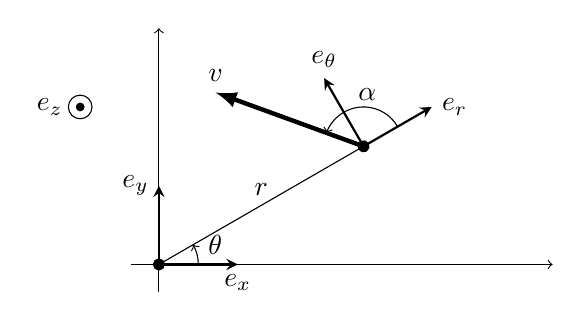
\begin{tikzpicture}
  \draw [-stealth,thick]  (0,0) -- (0,1) node [left] {$\vv{e_y}$};
  \draw [-stealth,thick]  (0,0) -- (1,0) node [below] {$\vv{e_x}$};
  \begin{scope}[shift={(-1,2)}]
    \draw (0,0)  circle(0.15);
    \fill (0,0) circle(1.6pt);
    \draw (-0.1,0) node[left]{$\vv{e_z}$};
  \end{scope}
  \draw [->] (-10pt,0) -- (5,0) ;
  \draw [->] (0,-10pt) -- (0,3) ;
   \pgfmathsetmacro{\THETA}{30}
   \pgfmathsetmacro{\ALPHA}{130}
   \pgfmathsetmacro{\cosTHETA}{cos(\THETA)}
   \pgfmathsetmacro{\sinTHETA}{sin(\THETA)}
   \pgfmathsetmacro{\cosALPHA}{cos(\ALPHA)}
   \pgfmathsetmacro{\sinALPHA}{sin(\ALPHA)}
  \draw [-stealth,thick,rotate=\THETA]  (3,0) -- (3,1) node [above] {$\vv{e_\theta}$};
  \draw [->,rotate=\THETA]  (3.5,0) arc (0:\ALPHA:0.5) node [above right=8pt] {$\alpha$};
  \draw [-stealth,thick,rotate=\THETA]  (3,0) -- (4,0) node [right] {$\vv{e_r}$};
  \draw [-latex,ultra thick,rotate=\THETA, \blueOrBlack]  (3,0) -- (3+2*\cosALPHA,2*\sinALPHA) node [above] {$\vv{v}$};
  \draw [rotate=\THETA] (0,0) -- (3,0) node [pos=0.5, above] {$r$};
  \filldraw [black,rotate=\THETA] (3,0) circle (2pt) node [below right] {$\ptM$};
  \filldraw [black] (0,0) circle (2pt) node [below left] {$\ptO$} ;
  \draw [->] (0.5,0) arc (0:\THETA:0.5) node [right=2pt] {$\theta$};
\end{tikzpicture}

% ====================================== %
\debutEntrainement
% ====================================== %

% ^^^^^^^^^^^^^^^^^^^^^^^^^^^^^^^^^^^^^^ %
%               Question                 %
% ^^^^^^^^^^^^^^^^^^^^^^^^^^^^^^^^^^^^^^ %

\begin{enonce}
Exprimer le moment cinétique du moustique $\ptM$ par rapport à $\ptO$ en fonction de $m$, $r$, $v$ et $\alpha$ \medskip
\\\mbox{} 
\end{enonce}

\reponse{$m\,r\,v\sin(\alpha)\,\vv{e_z}$}

\begin{corrige}
	Le vecteur vitesse s'écrit dans la base $(\vv{e_r}, \vv{e_\theta})$ comme $\vv{v} = v\left(\cos\alpha\,\vv{e_r} + \sin\alpha\,\vv{e_\theta}\right)$. Le produit vectoriel avec $\vv{\ptO\ptM}$ s'écrit alors
	\[
		\vv{\ptO\ptM} \wedge m\vv{v}
			= r\,\vv{e_r} \wedge m\,v\left(\cos\alpha\,\vv{e_r} + \sin\alpha\,\vv{e_\theta}\right)
			= m\,r\,v \sin\alpha\, \vv{e_r}\wedge\vv{e_\theta}.
	\]
\end{corrige}

% ************************************** %

% ====================================== %
\finEntrainement
% ====================================== %








% •••••••••••••••••••••••••••••••••••••• %
% •••••••••••••••••••••••••••••••••••••• %
\sectionFicheEntrainement{Moments d'inertie}
% •••••••••••••••••••••••••••••••••••••• %
% •••••••••••••••••••••••••••••••••••••• %



% ************************************** %
%             ENTRAÎNEMENT               %
% ************************************** %
% === Métadonnées sur l'entraînement === %

\titreEntrainementFacultatif	{Une porte d'entrée}
\hauteurLargeurCadreReponse		{8mm}{7cm}
\dureeResolutionFacultative		{1} % 1, 2, 3 ou 4
\typeEntrainement				{} % Newton ou QCM ou AN ou vide (exercice "normal")
\basiqueEtTransversal			{Y}
\nombreColonnesQuestions		{1} % vide, 1, 2, 3, \etc{}
\avecPlusieursQuestions			{N} % Y ou N
\initialisationEntrainement
% ====================================== %


% mmmmmmmmmmmmmmmmmmmmmmmmmmmmmmmmmmmmmmmmmmmmmmmmmmmmmmmmm %
% 		  Insertion d'une image en regard d'un texte
% mmmmmmmmmmmmmmmmmmmmmmmmmmmmmmmmmmmmmmmmmmmmmmmmmmmmmmmmm %
% --------------------------------------------------------- %
\pourcentageDeLaPartieAGauche   {0.55}
% --------------------------------------------------------- %
%                                                           %
% -------------------- Partie à gauche -------------------- %
%                                                           %
                                \initialisationPartieGauche % 
%                                                           %
%                                                           %
On considère une porte de masse $M$, de longueur $L$, de hauteur $h$ et d'épaisseur $e$ négligeable 
dont on veut calculer le moment d'inertie par rapport à l'axe vertical passant par $\ptO$ situé 
dans le coin inférieur gauche de la porte. 

La 
masse est répartie de manière homogène sur toute la porte, 
de sorte que chaque petit volume 
$\d{}V=\d{}x\,\d{}y\,\d{}z$
ait pour masse 
\[
\d{}m = \rho\,\d{}V
\]
avec $\rho = \frac{M}{Lhe}$. 

Dans cette configuration, le moment d'inertie s'écrit
\[
	I_\Delta = \iiint_{\text{porte}} x^2\,\d{}m
    = \rho\int_{0}^{L} \! x^2\,\d{}x \times \int_{0}^{e}\! \d{}y \times \int_{0}^{h}\! \d{}z.
\]

% --------------------------------------------------------- %
%                                                           %
% -------------------- Partie à droite -------------------- %
%                                                           %
                                \initialisationPartieDroite %
%                                                           %
%                                                           %
\begin{center}
\subimport{_images/}{porte_CBD_v2.tex}
\end{center}
% --------------------------------------------------------- %
                               \finalisationDuPartageDePage %					
% --------------------------------------------------------- %



% ====================================== %
\debutEntrainement
% ====================================== %

% ^^^^^^^^^^^^^^^^^^^^^^^^^^^^^^^^^^^^^^ %
%               Question                 %
% ^^^^^^^^^^^^^^^^^^^^^^^^^^^^^^^^^^^^^^ %

\bigskip

\begin{enonce}
Exprimer $I_\Delta$ en fonction de $M$ et $L$
\end{enonce}


\reponse{$\frac{1}{3}\,M\,L^2$}

\begin{corrige}
On calcule 
\begin{align*}
I_\Delta 
	&= \rho\int_{0}^{L} x^2\,\d{}x \times \int_{0}^{e}\d{}y \times \int_{0}^{h}\d{}z	\\
	&= \frac{M}{Lhe}\,\int_{0}^{L} x^2\,\d{}x \times e \times h\\
	&= \frac{M}{L}\,\int_{0}^{L} x^2\,\d{}x\\
    &= \left[\frac{M}{L}\,\frac{x^3}{3}\right]_{0}^{L}
    = \frac1{3}\,ML^2
\end{align*}
\end{corrige}

% ************************************** %

% ====================================== %
\finEntrainement
% ====================================== %



\newpage


% ************************************** %
%             ENTRAÎNEMENT               %
% ************************************** %
% === Métadonnées sur l'entraînement === %

\titreEntrainementFacultatif	{Un bâton de majorette}
\hauteurLargeurCadreReponse		{8mm}{7cm}
\dureeResolutionFacultative		{1} % 1, 2, 3 ou 4
\typeEntrainement				{} % Newton ou QCM ou AN ou vide (exercice "normal")
\basiqueEtTransversal			{Y}
\nombreColonnesQuestions		{1} % vide, 1, 2, 3, \etc{}
\avecPlusieursQuestions			{N} % Y ou N
\initialisationEntrainement
% ====================================== %



% mmmmmmmmmmmmmmmmmmmmmmmmmmmmmmmmmmmmmmmmmmmmmmmmmmmmmmmmm %
% 		  Insertion d'une image en regard d'un texte
% mmmmmmmmmmmmmmmmmmmmmmmmmmmmmmmmmmmmmmmmmmmmmmmmmmmmmmmmm %
% --------------------------------------------------------- %
\pourcentageDeLaPartieAGauche   {0.45}
% --------------------------------------------------------- %
%                                                           %
% -------------------- Partie à gauche -------------------- %
%                                                           %
                                \initialisationPartieGauche % 
%                                                           %
%                                                           %
On considère un bâton de masse $M$, de longueur $L$ et de section négligeable 
dont on veut calculer le moment d'inertie par rapport à son centre $\ptO$. 

La 
masse est régulièrement répartie uniquement selon une variable $x$, de sorte 
que le bout de bâton de longueur $\d{} x$ situé à une distance $x$ du 
centre ait pour masse $\d{}m = \frac{M}{L}\,\d{}x$. 

Pour une 
rotation par rapport à un axe $(\ptO z)$ orthogonal à l'axe $(\ptO x)$ du bâton, et passant par son centre, 
calculer en fonction de $M$ et $L$ l'expression du moment d'inertie. C'est-à-dire, calculer : 

% --------------------------------------------------------- %
%                                                           %
% -------------------- Partie à droite -------------------- %
%                                                           %
                                \initialisationPartieDroite %
%                                                           %
%                                                           %
\begin{center}
\subimport{_images/}{baton_CBD_v2.tex}
\end{center}
% --------------------------------------------------------- %
                               \finalisationDuPartageDePage %					
% --------------------------------------------------------- %



% ====================================== %
\debutEntrainement
% ====================================== %

% ^^^^^^^^^^^^^^^^^^^^^^^^^^^^^^^^^^^^^^ %
%               Question                 %
% ^^^^^^^^^^^^^^^^^^^^^^^^^^^^^^^^^^^^^^ %

\begin{enonce}
$
    I_\Delta = \int_{\text{bâton}} x^2\,\d{}m
    = \int_{-L/2}^{L/2} \frac{M}{L}\,x^2\,\d{}x =
$
\end{enonce}


\reponse{$\frac{1}{12}\,M\,L^2$}

\begin{corrige}
On calcule $I_\Delta = \int_{-L/2}^{L/2} \frac{M}{L}\,x^2\,\d{}x
    = \left[\frac{M}{L}\,\frac{x^3}{3}\right]_{-L/2}^{L/2}
    = \frac{M}{L}\times 2\,\frac{L^3/8}{3}
    = \frac1{12}\,ML^2
$.
\end{corrige}

% ************************************** %

% ====================================== %
\finEntrainement
% ====================================== %





% ************************************** %
%             ENTRAÎNEMENT               %
% ************************************** %
% === Métadonnées sur l'entraînement === %

\titreEntrainementFacultatif	{Une boule de bowling}
\hauteurLargeurCadreReponse		{12mm}{7cm}
\dureeResolutionFacultative		{2} % 1, 2, 3 ou 4
\typeEntrainement				{} % Newton ou QCM ou AN ou vide (exercice "normal")
\nombreColonnesQuestions		{1} % vide, 1, 2, 3, \etc{}
\avecPlusieursQuestions			{N} % Y ou N
\initialisationEntrainement
% ====================================== %

\hfil\includegraphics*{_images/coord_sph_global.pdf}

\bigskip

On considère une boule homogène de masse $M$ et de rayon $R$. 

Un élément de volume $\d{}V$ (valant 
$\d{}r \times r\,\d{}\theta \times r\sin\theta\,\d{}\varphi$ 
en coordonnées sphériques) correspond à une masse $\d{}m = \rho\,\d{}V$
avec $\rho = \dfrac{M}{\frac{4}{3}\pi\,R^3}$. 

Ces éléments de masse sont situés à une distance $r\sin\theta$ de l'axe $(\ptO z)$
de sorte que le moment d'inertie par rapport à cet axe puisse s'écrire
\[
	I_\Delta = \iiint_{\text{sphère}} (r\sin\theta)^2\,\d{}m	
	= \rho \int_{0}^{R} r^4\,\d{}r 
	\times \int_{0}^{\pi} \sin^3\theta\,\d{}\theta
	\times \int_{0}^{2\pi} \!\!\d{}\varphi.
\] 

% ====================================== %
\debutEntrainement
% ====================================== %

% ^^^^^^^^^^^^^^^^^^^^^^^^^^^^^^^^^^^^^^ %
%               Question                 %
% ^^^^^^^^^^^^^^^^^^^^^^^^^^^^^^^^^^^^^^ %

\begin{enonce}
	Exprimer $I_\Delta$ en fonction de $M$ et $R$
\end{enonce}


\reponse{$\frac{2}{5}\,M\,R^2$}

\begin{corrigeNewpage}
On calcule les trois intégrales indépendamment. 
On a bien sûr $\int_{0}^{2\pi} \d{}\varphi=2\pi$ et 
$\int_{0}^{R} r^4\,\d{}r = \frac{R^5}{5}$. 
Reste l'intégrale sur $\theta$ qui peux se résoudre avec un changement de
variable en $u = \cos\theta$ (qui donne $\d{}u = -\sin\theta\,\d{}\theta$) : 
\[
\int_0^\pi \sin^3\theta\,\d{}\theta 
	= \int_0^\pi \sin\theta\,(1 - \cos^2\theta)\,\d{}\theta
	= \int_1^{-1} - (1 - u^2)\,\d{}u
	= \left[u - \frac{u^3}{3}\right]_{-1}^{1}
	= \frac{4}{3}.
\]
Finalement, on obtient 
$I_\Delta = \dfrac{M}{\frac{4}{3}\pi\,R^3} 
	\times \frac{R^5}{5} \times \frac{4}{3}
	\times 2\pi 
	= \frac{2}{5}\,M\,R^2$.
\end{corrigeNewpage}
	
% ************************************** %

% ====================================== %
\finEntrainement
% ====================================== %



\newpage


% •••••••••••••••••••••••••••••••••••••• %
% •••••••••••••••••••••••••••••••••••••• %
\sectionFicheEntrainement{Moment d'une force}
% •••••••••••••••••••••••••••••••••••••• %
% •••••••••••••••••••••••••••••••••••••• %


% ************************************** %
%             ENTRAÎNEMENT               %
% ************************************** %
% === Métadonnées sur l'entraînement === %

\titreEntrainementFacultatif	{Fil accroché au mur}
\hauteurLargeurCadreReponse		{8mm}{2cm}
\dureeResolutionFacultative		{1} % 1, 2, 3 ou 4
\typeEntrainement				{} % Newton ou QCM ou AN ou vide (exercice "normal")
\nombreColonnesQuestions		{2} % vide, 1, 2, 3, \etc{}
\avecPlusieursQuestions			{Y} % Y ou N
\initialisationEntrainement
% ====================================== %

%% NB: exercices et codes des figures fournis par G. Burgunder



% mmmmmmmmmmmmmmmmmmmmmmmmmmmmmmmmmmmmmmmmmmmmmmmmmmmmmmmmm %
% 		  Insertion d'une image en regard d'un texte
% mmmmmmmmmmmmmmmmmmmmmmmmmmmmmmmmmmmmmmmmmmmmmmmmmmmmmmmmm %
% --------------------------------------------------------- %
\pourcentageDeLaPartieAGauche   {0.45}
% --------------------------------------------------------- %
%                                                           %
% -------------------- Partie à gauche -------------------- %
%                                                           %
                                \initialisationPartieGauche % 
%                                                           %
%                                                           %
On considère un mur auquel est accroché un filin qu'on tire depuis un point $\ptA$. Il s'agit de trouver le moment de la force $\vv{F}$ par rapport aux axes $(\ptO z)$ et $(\ptA z)$ en fonction de $F$, $\ell$ et~$\alpha$.

Calculer : 

% --------------------------------------------------------- %
%                                                           %
% -------------------- Partie à droite -------------------- %
%                                                           %
                                \initialisationPartieDroite %
%                                                           %
%                                                           %
\begin{center}
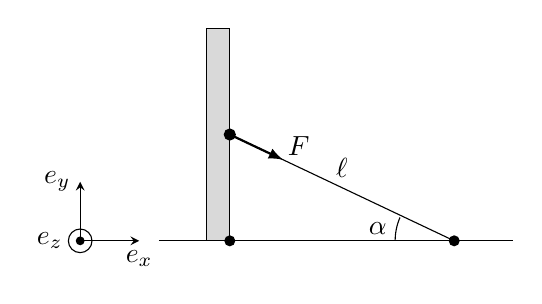
\begin{tikzpicture}
\begin{scope}[xshift = -1.75cm]
\draw[-stealth] (0,0) -- +(0.75,0) node[below]{$\vv{e_x}$};
\draw[-stealth] (0,0) -- +(0,0.75) node[left]{$\vv{e_y}$};
\draw (0,0)  circle(0.15);
\fill (0,0) circle(1.6pt);
\draw (-0.1,0) node[left]{$\vv{e_z}$};
\end{scope}
\begin{scope}[scale=1.5]
\draw (-0.5,0) -- +(3,0);
\filldraw[draw=black,fill=gray!30!white] (-0.1,0) rectangle (0.1,1.8);
\fill (0.1,0) circle(1.33pt) node[below]{$\ptO$};
\fill (2,0) circle(1.33pt) node[below]{$\ptA$};
\draw (2,0) -- (0.1,0.9) node[midway,above]{$\ell$};
\filldraw (0.1, 0.9) circle (1.33pt) node [above right] {$\ptM$} ;
\draw[thick,\blueOrBlack,-latex] (0.1,0.9) -- +(-25.34:0.5) node[above right=-2pt]{$\vv{F}$};
\draw (1.5,0) arc(180:156.66:0.5) node[midway,left]{$\alpha$};
\end{scope}
\end{tikzpicture}
\end{center}
% --------------------------------------------------------- %
                               \finalisationDuPartageDePage %					
% --------------------------------------------------------- %



% ====================================== %
\debutEntrainement
% ====================================== %

% ^^^^^^^^^^^^^^^^^^^^^^^^^^^^^^^^^^^^^^ %
%               Question                 %
% ^^^^^^^^^^^^^^^^^^^^^^^^^^^^^^^^^^^^^^ %

\begin{enonce}
	$\mathcal{M}_{\ptO z}(\vv{F})$
\end{enonce}

\reponse{$-\ell F\sin\alpha\cos\alpha$}

\begin{corrige}
	D'une part, on commence par déterminer l'expression du vecteur $\vv{F}$ dans la base $(\vv{e_x}, \vv{e_y})$. On a ici en notant $F$ la norme du vecteur: $\vv{F} = F\left(\cos\alpha\,\vv{e_x} - \sin\alpha\,\vv{e_y}\right)$. 
	
	D'autre part, en notant $\ptM$ le point d'action de $\vv{F}$, on a que $\vv{\ptO\ptM} = \ell\sin\alpha\,\vv{e_y}$.
	On peut alors calculer
	\[
		\vv{\mathcal{M}_{\ptO}}(\vv{F})
			= \vv{\ptO\ptM} \wedge \vv{F}
			= \ell\sin\alpha\,\vv{e_y} \wedge F\left(\cos\alpha\,\vv{e_x} - \sin\alpha\,\vv{e_y}\right)
			= \ell F\sin\alpha\cos\alpha\,(-\vv{e_z}).
	\]
\end{corrige}

% ************************************** %

% ^^^^^^^^^^^^^^^^^^^^^^^^^^^^^^^^^^^^^^ %
%               Question                 %
% ^^^^^^^^^^^^^^^^^^^^^^^^^^^^^^^^^^^^^^ %

\begin{enonce}
	$\mathcal{M}_{\ptA z}(\vv{F})$
\end{enonce}

\reponse{$0$}

% ====================================== %
\finEntrainement
% ====================================== %






% ************************************** %
%             ENTRAÎNEMENT               %
% ************************************** %
% === Métadonnées sur l'entraînement === %

\titreEntrainementFacultatif	{Une planche de cirque}
\hauteurLargeurCadreReponse		{8mm}{2cm}
\dureeResolutionFacultative		{2} % 1, 2, 3 ou 4
\typeEntrainement				{} % Newton ou QCM ou AN ou vide (exercice "normal")
\nombreColonnesQuestions		{3} % vide, 1, 2, 3, \etc{}
\avecPlusieursQuestions			{Y} % Y ou N
\initialisationEntrainement
% ====================================== %

%% NB: exercices et codes des figures fournis par G. Burgunder



% mmmmmmmmmmmmmmmmmmmmmmmmmmmmmmmmmmmmmmmmmmmmmmmmmmmmmmmmm %
% 		  Insertion d'une image en regard d'un texte
% mmmmmmmmmmmmmmmmmmmmmmmmmmmmmmmmmmmmmmmmmmmmmmmmmmmmmmmmm %
% --------------------------------------------------------- %
\pourcentageDeLaPartieAGauche   {0.45}
% --------------------------------------------------------- %
%                                                           %
% -------------------- Partie à gauche -------------------- %
%                                                           %
                                \initialisationPartieGauche % 
%                                                           %
%                                                           %
On considère une planche homogène de masse $m$ appuyée sur un cylindre. 

Calculer le moment du poids de cette planche par rapport aux divers points intéressants du système.

% --------------------------------------------------------- %
%                                                           %
% -------------------- Partie à droite -------------------- %
%                                                           %
                                \initialisationPartieDroite %
%                                                           %
%                                                           %
\begin{center}
\begin{tikzpicture}
	\begin{scope}[xshift = -2.5cm]
	\draw[-stealth] (0,0) -- +(0.75,0) node[below]{$\vv{e_x}$};
	\draw[-stealth] (0,0) -- +(0,0.75) node[left]{$\vv{e_y}$};
	\draw (0,0)  circle(0.15);
	\fill (0,0) circle(1.6pt);
	\draw (-0.1,0) node[left]{$\vv{e_z}$};
	\end{scope}
\begin{scope}
\draw (-0.75,0) -- +(4,0);

\begin{scope}[shift={(3,0)},rotate=-28.07]
\filldraw[draw=black,fill=gray!30!white] (0,0) rectangle +(-4.2,0.1) ;
\coordinate (G) at (-2.1, 0.05) ;
\filldraw (G) circle (2pt) node [left] {$\ptG$} ;
\end{scope}
\draw[thick,\blueOrBlack,-latex] (G) -- ++(0, -1) node[midway, right=-2pt]{$\vv{P}$};

\fill (0,0) circle(2pt) node[below]{$\ptI$};
\fill (3,0) circle(2pt) node[below]{$\ptA$};
\draw (0,0.75) circle(0.75) node[]{$+$} node[left]{$\ptO$};
%\filldraw[draw=black,fill=gray!30!white] (3,0) rectangle +(-28.07:-4.2);
\begin{scope}[shift = (61.92:0.25),shift={(3,0)}]
\draw[<->] (0,0) -- +(-28.07:-4.2) node[midway,above]{$L$};
\end{scope}
\draw[<->,shorten <= 3pt,shorten >= 3pt] (0,-0.15) -- +(3,0) node[midway,below]{$\ell$};
\draw[dotted] (0,0) -- (0,0.75) node[midway,left]{$R$} -- +(61.92:0.75);
\draw (2.4,0) arc(180:151.93:0.6) node[midway,left]{$\alpha$};
\end{scope}
\end{tikzpicture}
\end{center}
% --------------------------------------------------------- %
                               \finalisationDuPartageDePage %					
% --------------------------------------------------------- %


%%%%%%%%%%%%%%%%%%%%%%%%%%%%%%%%%%%%%%%%

% ====================================== %
\debutEntrainement
% ====================================== %


% ^^^^^^^^^^^^^^^^^^^^^^^^^^^^^^^^^^^^^^ %
%               Question                 %
% ^^^^^^^^^^^^^^^^^^^^^^^^^^^^^^^^^^^^^^ %

\begin{enonce}
	$\vv{\mathcal{M}_\ptA}(\vv{P})$
\end{enonce}

\reponse{$\frac{mgL}{2}\,\cos\alpha\,\vv{e_z}$}

\begin{corrige}
	Dans cette configuration, le bras de levier vaut $\frac{L}{2}\cos\alpha$ et le point fait tourner dans le sens trigonométrique autour de $\ptA$, de sorte que $\vv{\mathcal{M}_\ptA}(\vv{P}) = \frac{mgL}{2}\,\cos\alpha\,\vv{e_z}$.
\end{corrige}

% ************************************** %

% ^^^^^^^^^^^^^^^^^^^^^^^^^^^^^^^^^^^^^^ %
%               Question                 %
% ^^^^^^^^^^^^^^^^^^^^^^^^^^^^^^^^^^^^^^ %

\begin{enonce}
	$\vv{\mathcal{M}_\ptO}(\vv{P})$
\end{enonce}

\reponse{\small$-mg\left(\ell - \frac{L}{2}\cos\alpha\right)\,\vv{e_z}$}

\begin{corrige}
	Cette fois-ci, le poids fait tourner dans le sens horaire autour de $\ptO$ avec un bras de levier complémentaire du précédent de $\ell-\frac{L}{2}\cos\alpha$, d'où le résultat.
\end{corrige}

% ************************************** %

% ^^^^^^^^^^^^^^^^^^^^^^^^^^^^^^^^^^^^^^ %
%               Question                 %
% ^^^^^^^^^^^^^^^^^^^^^^^^^^^^^^^^^^^^^^ %

\begin{enonce}
	$\vv{\mathcal{M}_\ptI}(\vv{P})$
\end{enonce}

\reponse{\small$-mg\left(\ell - \frac{L}{2}\cos\alpha\right)\,\vv{e_z}$}

\begin{corrige}
	Même chose que précédemment, $\ptI$ et $\ptO$ étant à la verticale l'un de l'autre.
\end{corrige}

% ====================================== %
\finEntrainement
% ====================================== %








% •••••••••••••••••••••••••••••••••••••• %
% •••••••••••••••••••••••••••••••••••••• %
\sectionFicheEntrainement{Exercice récapitulatif}
% •••••••••••••••••••••••••••••••••••••• %
% •••••••••••••••••••••••••••••••••••••• %


% ************************************** %
%             ENTRAÎNEMENT               %
% ************************************** %
% === Métadonnées sur l'entraînement === %

\titreEntrainementFacultatif	{Basculement d'une barre en T}
\hauteurLargeurCadreReponse		{8mm}{5cm}
\dureeResolutionFacultative		{3} % 1, 2, 3 ou 4
\typeEntrainement				{} % Newton ou QCM ou AN ou vide (exercice "normal")
\nombreColonnesQuestions		{1} % vide, 1, 2, 3, \etc{}
\avecPlusieursQuestions			{Y} % Y ou N
\initialisationEntrainement
% ====================================== %

%% NB: exercices et codes des figures fournis par G. Burgunder



% mmmmmmmmmmmmmmmmmmmmmmmmmmmmmmmmmmmmmmmmmmmmmmmmmmmmmmmmm %
% 		  Insertion d'une image en regard d'un texte
% mmmmmmmmmmmmmmmmmmmmmmmmmmmmmmmmmmmmmmmmmmmmmmmmmmmmmmmmm %
% --------------------------------------------------------- %
\pourcentageDeLaPartieAGauche   {0.55}
% --------------------------------------------------------- %
%                                                           %
% -------------------- Partie à gauche -------------------- %
%                                                           %
                                \initialisationPartieGauche % 
%                                                           %
%                                                           %
On considère trois masses $m$ réparties aux trois sommets d'un triangle $\ptO\ptA\ptB$ isocèle en $\ptB$ et reliées par des tiges sans masse vérifiant 
\[
\ptO\ptA=\ptI\ptB=a.
\]

On note $\ptI$ le milieu du segment $[\ptO\ptA]$. 

On note $\ptG$ le centre de gravité des trois masses, qui est situé sur le segment $[\ptI\ptB]$ de sorte que $\ptG\ptB = \frac23\,a$. 

On notera $P$ et $F$ les normes des deux forces représentées sur le schéma.


% --------------------------------------------------------- %
%                                                           %
% -------------------- Partie à droite -------------------- %
%                                                           %
                                \initialisationPartieDroite %
%                                                           %
%                                                           %
\begin{center}
\begin{tikzpicture}
	\begin{scope}[xshift = -4cm]
	\draw[-stealth] (1,0) -- +(0.75,0) node[below]{$\vv{e_x}$};
	\draw[-stealth] (1,0) -- +(0,0.75) node[left]{$\vv{e_y}$};
	\draw (1,0)  circle(0.15);
	\fill (1,0) circle(1.6pt);
	\draw (-0.1+1,0) node[left]{$\vv{e_z}$};
	\end{scope}
%%%%%%%%%%%%%%%%%%%%%%%%%%%%%%%%%%%%%%%%
\pgfmathsetmacro{\ALPHA}{65}
\begin{scope}[rotate = \ALPHA]
% Les vecteurs de base
\draw[-stealth] (0,0) -- +(0.75,0) node[left=-2pt]{$\vv{e_X}$};
\draw[-stealth] (0,0) -- +(0,0.75) node[left=-2pt]{$\vv{e_Y}$};
% Les points intéressants
\coordinate (O) at (0, 0) ;
\coordinate (A) at (3, 0) ;
\coordinate (I) at (1.5, 0) ;
\coordinate (B) at (1.5, 3) ;
\coordinate (G) at (1.5, 1) ;
% Les deux lignes reliant les masses
\draw [thick] (O) -- (A) node [midway, below] {};
\draw [thick] (I) -- (B) node [midway, right] {};
% L'angle droit
\draw (I) ++ (0.1, 0) |- ++(-0.1, 0.1) ;
% Les positions des masses
\filldraw (O) circle (2pt) node [below right] {$\ptO$} node [yshift = -1mm, left] {$m$} ;
\filldraw (A) circle (2pt) node [above right] {$m$} node [below right=-2pt] {$\ptA$} ;
\filldraw (B) circle (2pt) node [above right] {$m$} node [below] {$\ptB$} ;
\filldraw (G) circle (1pt) node [above right=-2pt] {$\ptG$} ;
\filldraw (I) circle (1pt) node [below right] {$\ptI$} ;
\end{scope}
\draw[-latex,\blueOrBlack,thick] (B) -- +(-0.8,0) node[midway,above]{$\vv{F}$};
\draw[-latex,\blueOrBlack,thick] (G) -- +(0,-0.8) node[midway,left]{$\vv{P}$};
\draw (O) --++ (2.5, 0);
\draw [->] (0.5, 0) arc (0:\ALPHA:0.5) node [midway, right] {$\alpha$} ;
\end{tikzpicture}
\end{center}
% --------------------------------------------------------- %
                               \finalisationDuPartageDePage %					
% --------------------------------------------------------- %



% ====================================== %
\debutEntrainement
% ====================================== %

% ^^^^^^^^^^^^^^^^^^^^^^^^^^^^^^^^^^^^^^ %
%               Question                 %
% ^^^^^^^^^^^^^^^^^^^^^^^^^^^^^^^^^^^^^^ %

\begin{enonce}
	Écrire le vecteur $\vv{\ptO\ptB}$ dans la base $(\vv{e_X},\vv{e_Y})$
\end{enonce}

\reponse{$
	\frac{a}{2}\,\vv{e_X} + a\,\vv{e_Y}
	$}

\begin{corrige}
	On décompose $\vv{\ptO\ptB} = \vv{\ptO\ptI} + \vv{\ptI\ptB} = \frac{a}{2}\,\vv{e_X} + a\,\vv{e_Y}$.
\end{corrige}

% ************************************** %

% ^^^^^^^^^^^^^^^^^^^^^^^^^^^^^^^^^^^^^^ %
%               Question                 %
% ^^^^^^^^^^^^^^^^^^^^^^^^^^^^^^^^^^^^^^ %

\begin{enonce}
	Écrire le vecteur $\vv{\ptO\ptG}$ dans la base $(\vv{e_X},\vv{e_Y})$
\end{enonce}

\reponse{$
	\frac{a}{2}\,\vv{e_X} + \frac{a}{3}\,\vv{e_Y}
	$}

\begin{corrige}
	On décompose $\vv{\ptO\ptG} = \vv{\ptO\ptI} + \vv{\ptI\ptG} = \frac{a}{2}\,\vv{e_X} + \frac{a}{3}\,\vv{e_Y}$.
\end{corrige}

% ************************************** %

% ^^^^^^^^^^^^^^^^^^^^^^^^^^^^^^^^^^^^^^ %
%               Question                 %
% ^^^^^^^^^^^^^^^^^^^^^^^^^^^^^^^^^^^^^^ %

\begin{enonce}
	Écrire le vecteur $\vv{P}$ dans la base $(\vv{e_X},\vv{e_Y})$
\end{enonce}

\reponse{$P\left(-\sin\alpha\,\vv{e_X} -\cos\alpha\,\vv{e_Y}\right)$}

\begin{corrige}
	On a $\vv{P} = (\vv{P}\cdot\vv{e_X})\,\vv{e_X}
		+ (\vv{P}\cdot\vv{e_Y})\,\vv{e_Y}
		= P\left[\cos\left(\frac\pi2 + \alpha\right)\,\vv{e_X} + \cos(\pi+\alpha)\,\vv{e_Y}\right]
		= P\left(-\sin\alpha\,\vv{e_X} -\cos\alpha\,\vv{e_Y}\right)$.
\end{corrige}

% ************************************** %

% ^^^^^^^^^^^^^^^^^^^^^^^^^^^^^^^^^^^^^^ %
%               Question                 %
% ^^^^^^^^^^^^^^^^^^^^^^^^^^^^^^^^^^^^^^ %

\begin{enonce}
	Écrire le vecteur $\vv{F}$ dans la base $(\vv{e_X},\vv{e_Y})$
\end{enonce}

\reponse{$F\left(-\cos\alpha\,\vv{e_X} +\sin\alpha\,\vv{e_Y}\right)$}

\begin{corrige}
	On a $\vv{F} = (\vv{F}\cdot\vv{e_X})\,\vv{e_X}
		+ (\vv{F}\cdot\vv{e_Y})\,\vv{e_Y}
		= F\left[\cos\left(\pi + \alpha\right)\,\vv{e_X} + \cos\left(\frac{3\pi}2+\alpha\right)\,\vv{e_Y}\right]
		= F\left(-\cos\alpha\,\vv{e_X} + \sin\alpha\,\vv{e_Y}\right)$.
\end{corrige}

\begin{enonce}
	Calculer $\vv{\mathcal{M}_\ptO}(\vv{F})$
\end{enonce}

\reponse{\small$aF\left(\frac{\sin\alpha}{2} + \cos\alpha\right)\,\vv{e_z}$}

% ************************************** %

% ^^^^^^^^^^^^^^^^^^^^^^^^^^^^^^^^^^^^^^ %
%               Question                 %
% ^^^^^^^^^^^^^^^^^^^^^^^^^^^^^^^^^^^^^^ %

\begin{enonce}
	Calculer $\vv{\mathcal{M}_\ptO}(\vv{P})$
\end{enonce}

\reponse{\small$
aP\left(-\frac{\cos\alpha}2 + \frac{\sin\alpha}3\right)\,\vv{e_z}
$}

% ************************************** %

% ^^^^^^^^^^^^^^^^^^^^^^^^^^^^^^^^^^^^^^ %
%               Question                 %
% ^^^^^^^^^^^^^^^^^^^^^^^^^^^^^^^^^^^^^^ %

\begin{enonce}
	 En supposant qu'il y ait équilibre entre les deux moments, déterminer l'expression $\tan(\alpha)$ dans ce cas.\\
	 \mbox{}
\end{enonce}

\reponse{$\frac{3P - 6F}{3F + 2P}$}

\begin{corrige}
	Pour qu'il y ait équilibre, la somme des deux moments doit s'annuler. Les deux étant suivant $\vv{e_z}$, on doit avoir
	\[
		aF\left(\frac{\sin\alpha}{2} + \cos\alpha\right)
		+ aP\left(-\frac{\cos\alpha}2 + \frac{\sin\alpha}3\right) = 0.
	\]
	En divisant par $a\cos\alpha$, il vient
	\[
		\frac{F\tan\alpha}{2} + F - \frac{P}{2} + \frac{P\tan\alpha}{3} = 0.
	\]
	On obtient donc
	\[
		\tan\alpha = \frac{\frac{P}{2} - F}{\frac{F}{2}+\frac{P}{3}} = \frac{3P - 6F}{3F + 2P}.
	\]
\end{corrige}

% ************************************** %

% ====================================== %
\finEntrainement
% ====================================== %



% -------------------------------------- %
%   Affichage des réponses mélangées     %
% -------------------------------------- %
\afficheReponsesMelangees
% -------------------------------------- %

%%%%%%%%%%%%%%%%%%%%%%%%%%%%%%%%%%%%%%%%%%
\finFicheEntrainement                    %
%%%%%%%%%%%%%%%%%%%%%%%%%%%%%%%%%%%%%%%%%%


% ======================================================= %
% ============== Gestion de la compilation ============== %
% ======================================================= %
\ifdefined\mainIsLoaded\else
\printReponsesEtCorriges
\end{document}\fi
% ======================================================= %
% ======================================================= %
